\documentclass[12pt,a4paper]{article} 
\usepackage[portuguese]{babel} \usepackage[utf8]{inputenc}
\usepackage{amsmath} 
\usepackage{graphicx}
\usepackage{booktabs}
\usepackage{pgfplots}
\usepackage{tikz}
\usepackage{float}
\pgfplotsset{compat=1.15}
\begin{document}
\setcounter{figure}{1}
\setcounter{section}{2}
\setcounter{page}{6}
\section{Relatório}
\subsection{Introdução}
Existem três modos de operação de um transistor bipolar de junção; corte, triodo e saturação. No entanto, para aplicações 
em que o dispositivo precisa atuar como chave, utilizamos apenas dois modos: corte e saturação. O transistor em corte
significa que a chave está aberta, i.e.\ não passa corrente,  e fechada, i.e. há passagem de corrente entre coletor e emissor, em saturação.

\begin{figure}[htpb]
  \centering
  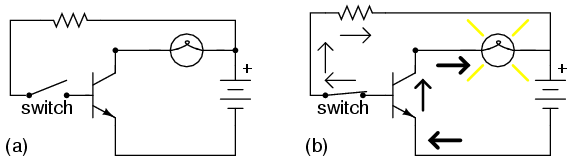
\includegraphics[width=0.8\linewidth]{./img/switch.png}
  \caption{Transistor bipolar utilizado como um \emph{switch} para controlar uma lâmpada.}
  \label{fig:divisortensao}
\end{figure}

A principal diferença entre o modo de saturação o modo de
condução triodo é o ganho ao qual o transistor opera, ou seja, a relação entre correntes de base e
coletor, e a queda de tensão, $V_{CE}$ sobre ele. Esses limites podem prontamente serem encontrados na folha de dados
de cada componente.

Nesta prática, para o controle do modo de operação, será feita uma montagem que permite regular
a tensão de entrada na base. Este controle é essencial pois sabe-se que a corrente de base é quem controla a passagem de portadores minoritários 
entre emissor e coletor. Desta forma, os circuitos devem ser apropriadamente modelados e dimensionados  para que possam alternar entre 
saturação e corte, atuando apropriadamente como chave.

\begin{figure}[htpb]
  \centering
  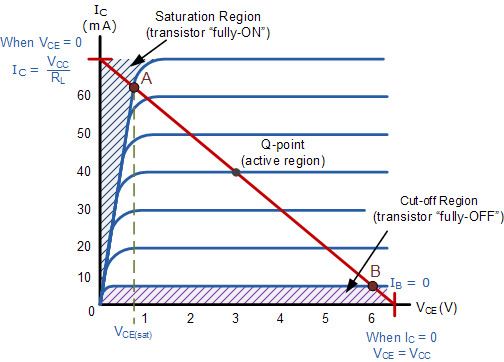
\includegraphics[width=0.8\linewidth]{./img/tran27.jpeg}
  \caption{A área sombreada, em rosa, no fundo da curva representa a região de corte do transistor enquanto a área sombreada, em azul, representa a região de saturação do transistor.}
  \label{fig:transgraf}
\end{figure}


Esta chave pode atuar no controle de lâmpadas, relês e até mesmo motores.
Vale ressaltar, que transistores também tem sido amplamente utilizados em circuitos digitais, 
e o entendimento  de como um transistor pode vir atuar como uma chave, e como projetar 
um circuito para que isto seja possíve, pode 
vir a ser de extrema importância para o entendimento
destas aplicações digitais atuais. 

\newpage
\subsection{Análises}
Montou-se o circuito da Figura~1 e calculou-se o valor da resistência necessária 
ao  potênciometro para que corrente da base fosse $30 \mu A$.  Fazendo uso da lei
de Ohm, pôde-se concluir que deve-se ajustar o potenciômetro para um valor igual a
$31.4 \Omega$. Feito este ajuste, mediu-se $V_{BE}$, $V_{CE}$ e $I_{C}$ com um multímetro. Mudou-se o resistor, $R_{C}$, e recalculou-se estes 
mesmos parâmetros. Estas medidas geraram a Tabela~1. 
      \begin{table}[H]
        \centering
        \caption{Medidas de tensão e corrente para diferentes valores de $R_{c}$ do circuito da Figura~1.}
        \label{tab:ex1}
        \begin{tabular}{c c c c c}
                          \\ \toprule
        $R_C$ (k$\Omega$)  & $V_{BE}$ (V) & $V_{CE}$ (V) & $I_C$ (mA) & Modo     \\ \midrule
        10                 & 0.646        & 72.2m        & 1.01       & Saturado \\ \midrule
        1                  & 0.696        & 1.295        & 8.837      & Triodo   \\ \bottomrule
        \end{tabular}
        \end{table}

        Para o segundo experimento, montaram-se os circuitos da Figura~2 e Figura~3, com o potenciômetro
        ajustado conforme anteriormente, e, com o multímetro digital, foram realizadas medidas de $V_{BE}$,
        $e_B$, $V_{CE}$ e $I_C$ para traçar a reta de carga, que está representada na \ref{fig:carga}.

      \begin{table}[H]
        \centering
        \caption{Medidas de tensão e correntes para o transistor cortado e reverso no experimento 2.}
        \label{tab:ex2}
        \begin{tabular}{ c c c c c }
                         \\ \toprule
                   & $V_{BE}$ (mV) & $V_{CE}$ (V) & $I_C$ (mA) & $I_{B}(\mu A)$ \\ \midrule
           Cortado & 31.5          & 9.97         & 0          & 0\\ \midrule 
           Reverso & -92.8         & 9.97         & 0 & -2          \\ \bottomrule
        \end{tabular}
        \end{table}

        \begin{figure}[htpb]
          \centering
          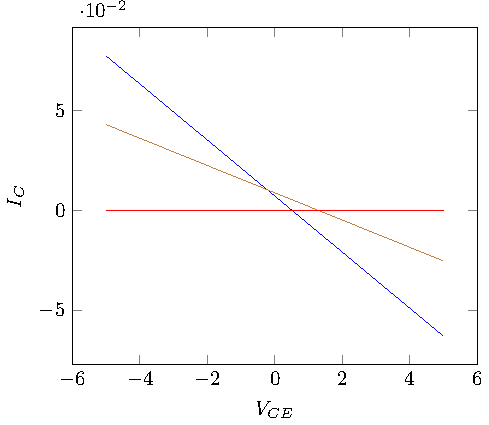
\includegraphics[width=0.8\linewidth]{./img/reta.pdf}
          \caption{Retas de carga para as várias configurações do circuitos. A reta azul 
            diz respeito ao transistor operando em região de saturação (resistor $10k$), a reta
          marrom diz respeito ao transistor operando em região de triodo (resistor $1k$). As demais retas
        sobrepostas são da operação em corte e reverso.}
          \label{fig:carga}
        \end{figure}

        Da Tabela~2 e do datasheet, concluiu-se, que no primeiro caso do experimento 2,  o transistor está em corte, pois não fluí corrente do coletor
para o emissor. E de forma similar, podemos concluir que o transistor está reversamente polarizado no segundo caso do experimento 2, pois 
corrente saí de sua base.

No último experimento, montou-se o circuito da Figura~4 e aplicou-se um sinal senoidal de frequência $3$kHz e  amplitude $3$V. Usando 
um multímetro digital, mediu-se a tensão de base e coletor do transistor. Repetiram-se as medidas retirando o sinal de entrada. O led
apenas se manteve aceso quando havia entrada senoidal. 
Os dados resultaram na Tabela~3.

\begin{table}[htpb]
  \centering
  \caption{Valores de tensão para o circuito de sinalização.}
  \label{tab:label}
  \begin{tabular}{c c c}
    \\ \toprule
    &$V_{B}$ (V) &$V_{C}$   \\ \midrule
    Com tensão senoidal & 0.734& 0.0653 \\ \midrule 
    Sem tensão senoidal & 0& 8.58 \\ \bottomrule
  \end{tabular}
\end{table}
\subsection{Discussões}
Consultando o Datasheet do transistor BC-237 podemos notar que um $V_{CE}$ menor que 0.2V e $V_{BE}>0.6$ define o estado de saturação. Desta forma
o circuito com resistor $10k\Omega$, se apresenta saturado, pois seu $V_{CE}=72.2mV$. A partir desta mesma condição, define-se que 
a configuração de $1k\Omega$ está em triodo, pois seu $V_{CE}=1.295>>0.2$. Percebe-se a partir da reta de carga  que, conforme aumenta-se
o valor de $R_C$, diminui-se o valor de $I_C$, até um ponto de saturação,
aonde seu ganho cai drasticamente.

Montou-se o circuito da Figura~2. O circuito  foi montado com
o objetivo de deixar o transistor na região de corte. 
A condição para que um transistor bipolar esteja na região de corte é que $V_{BE}<0.6$, pois a partir dessa tensão, a junção base emissor
fica cortada. 

Em seguida, monta-se o circuito da Figura~3, com o objetivo de
se polarizar reversamente a junção base emissor. Os resultados deste experimentos foram
dispostos na Tabela 2 e no gráfico da Figura 6. Em ambos os casos, a corrente de coletor
$I_C$ foi igual a 0. Na situação de corte, ambas junções base coletor e base emissor ficaram
cortadas, não havendo corrente de base, $I_B$, nem corrente de coletor $I_C$, conforme os
dados da Tabela 2. Porém, na situação de polarização reversa, há corrente entrando no emissor
e saindo pela base,no entanto,  não houve presença de corrente de coletor no processo.

No último experimento, foi montado o circuito da Figura~4.  
Assim como  os demais circuitos, este está na configuração de emissor comum. O circuito 
foi montado para que o estado do transistor alterne entre a região de corte a região de saturação. 
Para valores suficientes de entrada (ao menos $0.6$ Volts), o diodo $D_2$
passa a conduzir corrente, e parte dessa corrente entra na base do transistor. Isso faz com
que haja uma corrente no coletor do transistor, que ocasiona uma queda de tensão no
LED, acendendo-o. No caso em que retirou-se a entrada senoidal, observou-se que $V_B$ se igualou a zero 
e que o LED apagou-se. Isso ocorreu pois os resistores ligados a base do transistor serviram 
como resistores de pull-down, fazendo a tensão se igualar a terra. Dessa forma, 
$V_{BE}$ permaneceu zero, o que fez com que o
transistor ficasse em corte, ou seja, deixou de conduzir corrente, 
apagando o LED.

\newpage
\subsection{Conclusão}
Com a finalidade de aprender mais a respeito de transistores bipolares como chaves,
montou-se três circuitos distintos. No primeiro circuito fizemos uso de um potenciômetro 
para que pudessemos ajustar a corrente que entrava na base. Neste circuito, foi possível 
enteder o funcionamento do transistor operando no modo de saturação.

No segundo caso, montou-se um circuito em que o transistor operava na região de corte, pois
a configuração garantiu que a tensão entre base e emissor fosse menor que $0.6V$, o 
que resultou em correntes de base  corrente de coletor nulas. 

Finalmente, no terceiro circuito, foi possível observar uma configuração que alternava 
entre as regiões de corte e saturação do resistor. O circuito com um sinal de entrada 
acendia o LED. Quando o sinal de entrada era removido, o transistor voltava para corte 
e apagava o LED.

Assim, está prática de forma simples conseguiu demonstrar o funcionamento de cada 
um dos modos do transistor e como pode-se construir uma chave através do transistor
bipolar de junção.
\end{document}
